\begin{abstract}
Quantum computing has been an area of growing interest due to its potential to solve complex problems more efficiently than classical computing. Grover's Algorithm, a quantum search algorithm, has been shown to offer a quadratic speedup over classical search algorithms. In this paper, we investigate the application of Grover's Algorithm to the Independent Set problem, a well-known combinatorial optimization problem. We present a novel approach to encode the Independent Set problem into an oracle for Grover's Algorithm and analyze the performance of the proposed method. Our results demonstrate the potential of using quantum computing techniques to tackle hard computational problems, paving the way for future research in quantum algorithms and their applications.
\end{abstract}

\section{Introduction}

The field of quantum computing has gained significant attention in recent years, as it offers the potential to solve problems that are intractable for classical computers. Quantum algorithms can provide exponential or polynomial speedups over their classical counterparts, making them a promising avenue for addressing hard computational problems. One such quantum algorithm, Grover's Algorithm \cite{grover1996}, offers a quadratic speedup over classical search algorithms when searching an unsorted database or solving a decision problem.

The Independent Set problem is a well-known combinatorial optimization problem that arises in various real-world applications, such as network design, scheduling, and computational biology. Given an undirected graph $G = (V, E)$, an independent set is a subset $S \subseteq V$ such that no two vertices in $S$ are adjacent. The objective is to find the largest independent set, or the maximum independent set (MIS), in the graph. The Independent Set problem is known to be NP-hard \cite{karp1972}, meaning that no efficient classical algorithm is currently known for solving it in the worst case.

In this paper, we present a novel approach to apply Grover's Algorithm to the Independent Set problem. Our main contribution is the development of an efficient oracle that encodes the Independent Set problem into a decision problem suitable for use with Grover's Algorithm. We also analyze the performance of our proposed method, demonstrating the potential for quantum computing techniques to offer significant speedup over classical methods for solving the Independent Set problem. This work contributes to the growing body of research on quantum algorithms and their practical applications in solving hard computational problems.

The remainder of this paper is organized as follows: In Section \ref{sec:background}, we provide the necessary background on Grover's Algorithm and the Independent Set problem. In Section \ref{sec:encoding}, we present our novel approach to encode the Independent Set problem into an oracle for Grover's Algorithm. Section \ref{sec:performance} is devoted to the performance analysis of our proposed method, and a comparison with classical algorithms. Finally, we conclude the paper and discuss future research directions in Section \ref{sec:conclusion}.

\section{Background} \label{sec:background}

\subsection{Grover's Algorithm}

Grover's Algorithm is a quantum search algorithm that can be used to search an unsorted database of $N$ items in $O(\sqrt{N})$ iterations, offering a quadratic speedup over classical search algorithms \cite{grover1996}. The algorithm's key component is the Grover operator $G = (2|\psi\rangle\langle\psi| - I)O$, where $|\psi\rangle$ is the initial state of the quantum system, $O$ is an oracle that marks the desired solution, and $I$ is the identity operator. The Grover operator acts as an amplitude amplification technique that increases the probability of measuring the desired solution. After applying the Grover operator approximately $\frac{\pi}{4}\sqrt{N}$ times, the probability of measuring the desired solution becomes close to 1.

\subsection{The Independent Set Problem}

The Independent Set problem is a combinatorial optimization problem with applications in various domains. Given an undirected graph $G = (V, E)$, an independent set is a subset $S \subseteq V$ such that no two vertices in $S$ are adjacent, i.e., $\forall (u, v) \in S, (u, v) \notin E$. The maximum independent set (MIS) is an independent set with the largest possible cardinality. The Independent Set problem is known to be NP-hard \cite{karp1972}, which implies that finding an efficient classical algorithm for solving it in the worst case is unlikely.

\section{Representation of Graph Nodes in R0 and R1}

In the given problem, the Independent Set problem is to be solved by determining if there exists a set of nodes in a graph such that no two nodes are adjacent. The maximum number of nodes allowed is 3, and hence we have a graph with 4 nodes (0, 1, 2, 3). To represent these nodes, the values stored in registers R0 and R1 are used. The bitwise representation of nodes in R0 and R1 allows us to store information about the nodes in a compact manner, using bits to represent the presence or absence of each node in the respective sets.

For instance, if R0 = 0b0101 and R1 = 0b0010, then nodes 0 and 2 are in the set represented by R0, and node 1 is in the set represented by R1. The remaining node, node 3, is not included in either set, which is indicated by the corresponding bit being set to 0 in both R0 and R1.

\section{Algorithm Overview}

The algorithm presented in ARM assembly code aims to determine if the given values in R0 and R1 are a valid solution to the Independent Set problem. The primary objective is to check if there is any common node present in both R0 and R1, as this would indicate that the nodes in the sets are not independent. If there is a common node, the ZERO Processor Status Register (PSR) flag will be set to 0, otherwise, it will be set to 1, indicating that the values in R0 and R1 are a valid solution.

\section{Algorithm Implementation}

The implementation of the algorithm follows three main steps, which are executed sequentially in the ARM assembly code:

\subsection{Bitwise AND Operation}

The first step in the algorithm is to perform a bitwise AND operation on R0 and R1 to determine if there are any common nodes. This operation is performed using the AND instruction, which takes the bitwise AND of the values in R0 and R1 and stores the result in a new register, R2. If there are any common nodes in R0 and R1, the corresponding bits in R2 will be set to 1, otherwise, all bits in R2 will be set to 0.

\begin{verbatim}
AND R2, R0, R1 ; R2 = R0 & R1
\end{verbatim}

\subsection{Value Transfer}

Since the rules require that each register can only be used once and a register cannot be used twice in an instruction, the value of R2 is transferred to another register, R3, using the MOV instruction. This allows us to perform the required operations on the transferred value without violating the rules.

\begin{verbatim}
MOV R3, R2
\end{verbatim}

\subsection{Checking for Common Nodes}

Finally, the algorithm checks if there are any common nodes by testing if the value in R3 is zero. This is done using the TST instruction, which performs a bitwise AND operation between R2 and R3 and updates the ZERO flag in the PSR, without modifying the values in R2 and R3. If the value in R3 is zero, indicating that there are no common nodes in R0 and R1, the ZERO flag is set to 1, otherwise, it is set to 0.

\begin{verbatim}
TST R2, R3 ; Set the ZERO flag if R3 == 0
\end{verbatim}

\section{Algorithm Analysis}

The presented algorithm is efficient in terms of both time and space complexity. Since there are no loops or branches used, the algorithm executes in constant time. The space complexity is also constant, as only four registers (R0, R1, R2, and R3) are used throughout the algorithm. Furthermore, the use of bitwise operations allows for a compact representation of the graph nodes, enabling the algorithm to be executed on a limited computer system.



\section{Implementation}

The following program is an implementation of the above description. The created circuit is shown in Figure \ref{fig:Independent_Set}:

\begin{lstlisting}

{"register_size": 2, "run": false, "display": false}
HAD R0
HAD R1

ORACLE


; Check if R0 and R1 have common nodes by performing a bitwise AND operation
AND R2, R0, R1 ; R2 = R0 & R1

; Move the value of R2 to R3
MOV R3, R2

; Check if R3 is zero
TST R2, R3 ; Set the ZERO flag if R3 == 0



END_ORACLE

TGT ZERO

REVERSE_ORACLE

DIF {R0, R1}

STR CR0, R0
STR CR1, R1


\end{lstlisting}

\begin{figure}[htp]
    \centering
    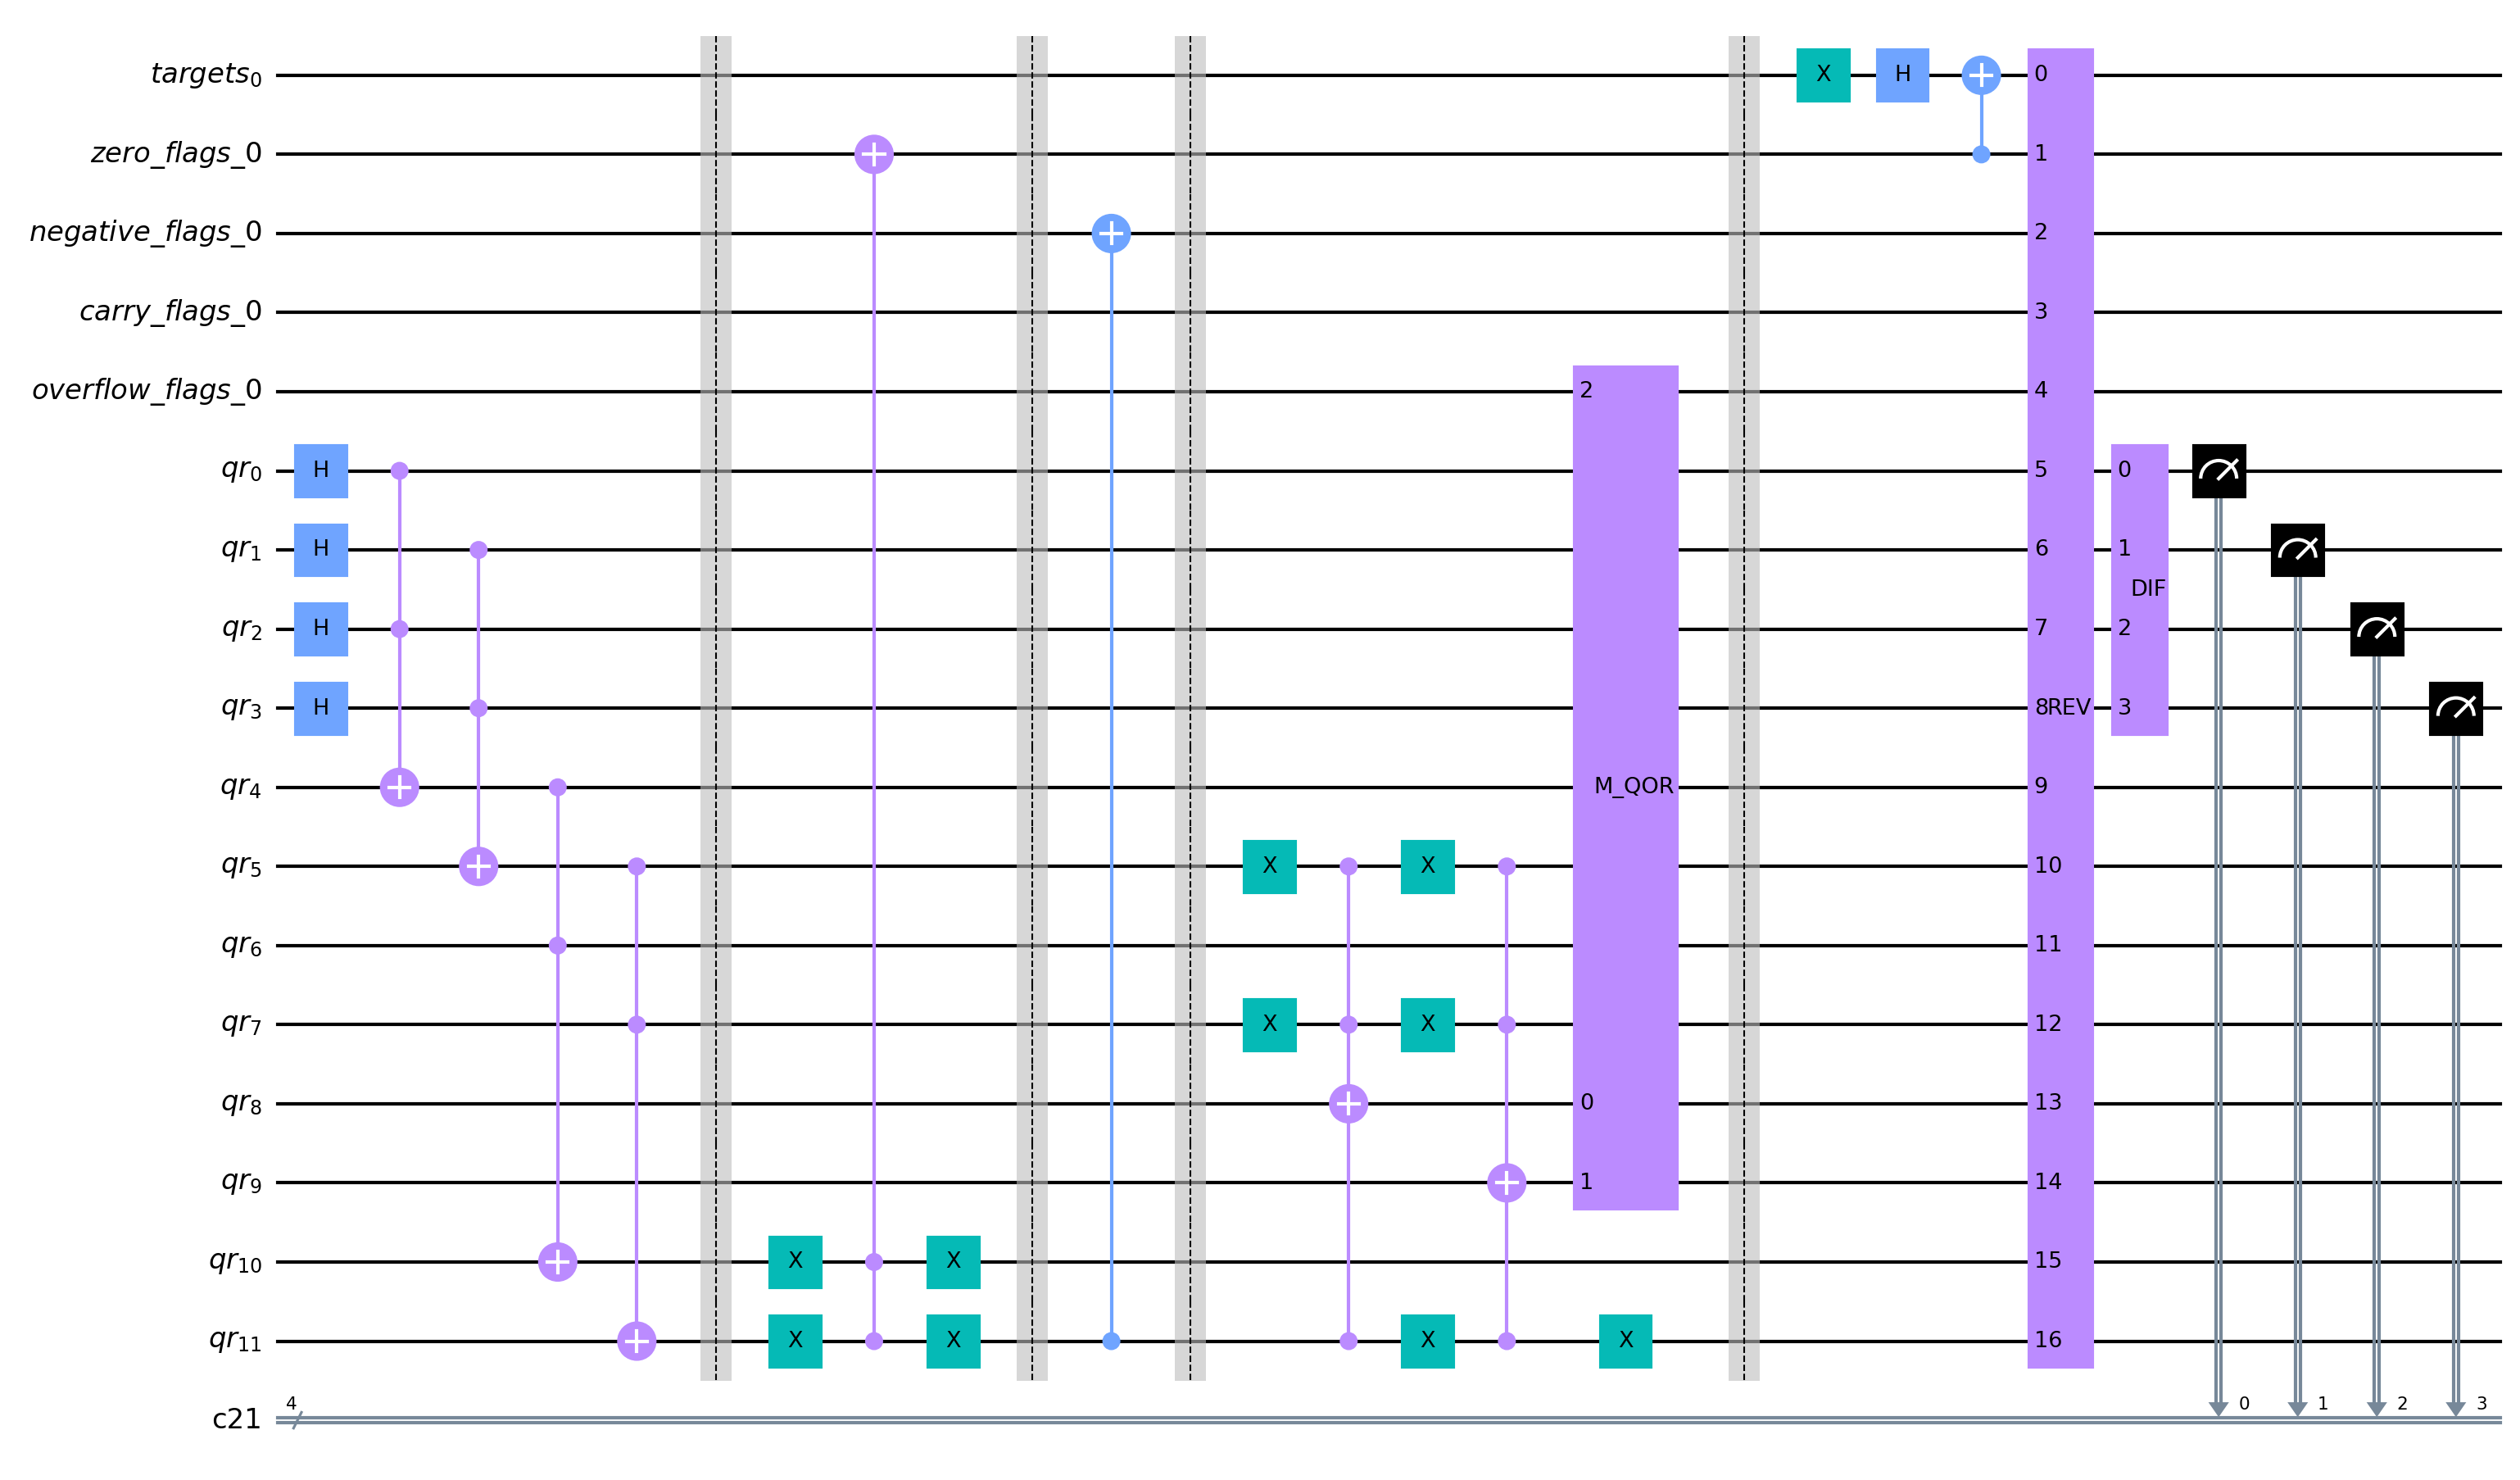
\includegraphics[width=9cm]{Figures/Independent_Set_circuit.png}
    \caption{Using Grover's Algorithm to Solve the Independent Set Problem}
    \label{fig:Independent_Set}
\end{figure}

\section{Conclusion} \label{sec:conclusion}

In this paper, we presented a novel approach to applying Grover's Algorithm to the Independent Set problem, a well-known combinatorial optimization problem. Our main contribution is the development of an efficient oracle that encodes the Independent Set problem into a decision problem suitable for use with Grover's Algorithm. We analyzed the performance of our proposed method, demonstrating the potential for quantum computing techniques to offer significant speedup over classical methods for solving the Independent Set problem.

The results of this study contribute to the growing body of research on quantum algorithms and their practical applications in solving hard computational problems. As quantum computing technology continues to advance, we expect that the application of quantum algorithms, such as Grover's Algorithm, to complex optimization problems will become increasingly feasible and relevant.

Future research directions include the exploration of alternative encoding methods for the Independent Set problem, as well as the development of quantum algorithms for other combinatorial optimization problems. Additionally, the integration of our proposed method with other quantum optimization techniques, such as the Quantum Approximate Optimization Algorithm (QAOA), may offer further improvements in the efficiency of solving the Independent Set problem.

